\newpage
\section{Model Synchronization}
\genHeader

At this point you have successfully created a trio of rules that can transform a \texttt{box} (with an undetermined number of \texttt{partition}s which can
contain an unknown number of \texttt{card}s) \emph{forwards} into a single \texttt{dictionary} able to store an unlimited number of \texttt{entry} elements. 
But what if you wanted to quickly made a change to either model, such as adding a \texttt{card} in a \texttt{partition}, or removing an \texttt{entry} from a
\texttt{Dictionary}? You don't want to have to run the ENTIRE transformation again. After all, you're only changing one small thing - the rest of the model
doesn't need to be updated.

This is where synchronization comes in handy. It uses the graph triple derived from the original transformation - the source, correspondence, and target
metamodels - and updates all three as needed. It can be used in either direction. Let's try this out. In the forward direction, from \texttt{Box} to
\texttt{Dictionary}, let's add a fourth paritition to \texttt{Partition 2}.

Now, we don't want to change the source model directly. Instead, we want to load it first, make the modification, and go from there. We want to generate a new,
updated instance of source.

\begin{itemize}

\item[$\blacktriangleright$] You are able to implement any updates/changes via SDMs, but here we'll just use basic java implementation, so complete the empty
override \texttt{changeSrc} method as depicted in Fig.~\ref{eclipse:changeSrc}.

\begin{figure}[htbp]
\begin{center}
  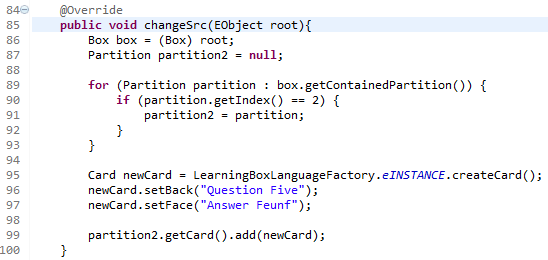
\includegraphics[width=0.8\textwidth]{eclipse_changeSrc}
  \caption{changing the source model}
  \label{eclipse:changeSrc}
\end{center}
\end{figure}

\item[$\blacktriangleright$] As you can see, \texttt{root} refers to the original root structure of the source model we loaded, which is a \texttt{Box}. We also
initalize partition2 so that we can make changes. We match to the correct one (for:each). Factory handles everything there is to do with box, so create a new
card, and set its values. Add the card to the partition, and you're done!

\item[$\blacktriangleright$] Add a new method, \texttt{synchForward}, and complete it as depicted in Fig.~\ref{eclipse:SynchForwardMethod}. 

\begin{figure}[htbp]
\begin{center}
  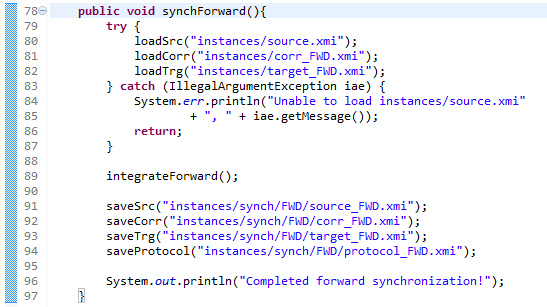
\includegraphics[width=\textwidth]{eclipse_synchForwardMethod}
  \caption{forward synchronization}
  \label{eclipse:SynchForwardMethod}
\end{center}
\end{figure}

\item[$\blacktriangleright$] You'll notice that its nearly identical to the original \texttt{performForward}. The difference here however is that you're loading
the original triple, \texttt{source.xmi}, and its generated \texttt{corr\_FWD.xmi} and \texttt{target\_FWD.xmi} in order to keep them consistent.

\item[$\blacktriangleright$] We'll come back to the command in a moment, but \texttt{integrateForward} commits any changes, and you'll need to persist all
changes in each piece, needing to save the source, target, and the minor update's relevant correspondence and protocol. These files will be significantly
smaller than the originals as they only reflect the immediate changes you made. Here we save them in a different location so that you may compare the
differences, and understand how synchronization works but you can, of course, decide to overwrite the original files. 


\item[$\blacktriangleright$] Finally, add the the following statements to \texttt{main}, then run \texttt{TGGMain}.

\begin{figure}[htbp]
\begin{center}
\begin{lstlisting}[language=Java,backgroundcolor=\color{white}, keywordstyle={\bfseries\color{purple}}]
helper = new TGGMain();
helper.synchForward();
\end{lstlisting}
\caption{add this to \texttt{main}}
  \label{code:synchForward}
\end{center}
\end{figure}

\item[$\blacktriangleright$] Navigate to ``instances/synch/FWD/'' and inspect the new \texttt{source} and \texttt{target} models. 
Is the fifth Card now in both source and target?

\item[$\blacktriangleright$] Compare these two new models to the original source and targets in ``instances/'' You'll notice they don't match. The new card was
added to source, but persisted in this other folder. 

\item[$\blacktriangleright$] Run the integrator on the correspondence. You'll notice that you can't go very far. in fact, the ONLY thing the corr will
show is the creation of this single card. It doesn't run through the entire transformation because the only thing that was modified or changed was this. Only
the items reflected are re-generated.

\item[$\blacktriangleright$] Lets try synchronizing in the opposite direction, from Dictionary to Box. Let's remove \texttt{Entry} `One: Eins,' and add `Five:
Feunf.' complete \texttt{changeTrg()} as shown in Fig.~\ref{eclipse:changeTrg}.

\begin{figure}[htbp]
\begin{center}
  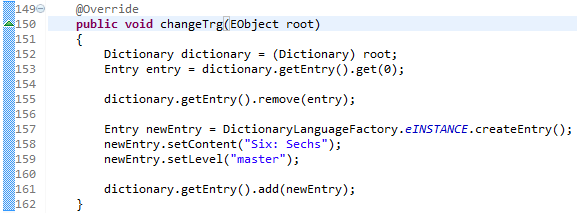
\includegraphics[width=0.8\textwidth]{eclipse_changeTrg}
  \caption{Modifying target model}
  \label{eclipse:changeTrg}
\end{center}
\end{figure}

\item[$\blacktriangleright$] Nearly identical to \texttt{synchForward}, create a new method \texttt{synchBackwards} and complete it as depicted in
Fig.~\ref{eclipse:SynchBackwardMethod}.

\begin{figure}[htbp]
\begin{center}
  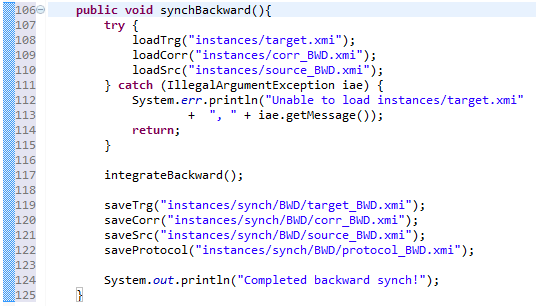
\includegraphics[width=\textwidth]{eclipse_synchBackwardMethod}
  \caption{synch backwards}
  \label{eclipse:SynchBackwardMethod}
\end{center}
\end{figure}

\item[$\blacktriangleright$] Finally, analogously to how you did in the forward direction, re-initalize \texttt{helper} and call
\texttt{helper.synchBackward()}. Your final \texttt{Main} method should come to resemble Fig.

\begin{figure}[htbp]
\begin{center}
  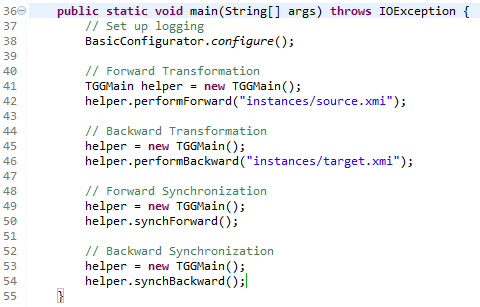
\includegraphics[width=\textwidth]{eclipse_TGGSynchMain}
  \caption{Final Main method}
  \label{eclipse:TGGSynchMain}
\end{center}
\end{figure}

\item[$\blacktriangleright$] Inspect the new files in ``instances/synch/BWD/.'' You'll notice in \texttt{target.xmi} that the \texttt{one} entry was removed,
and \texttt{Five} was added, but there's no \texttt{four}. this is because you ran off the ORIGINAL, non-updated target. We encourage you to experiment and try
to create a streamlined process, from original transformation to any synchronization updates you may make, forwards or backwards.

\item[$\blacktriangleright$] On a final note, lets run the integrator one more time. Notice how it doesn't show the deletion of the first card? Recall that
the rules of any TGG are by definition, monotoic. They only speciy the consistency relation, which is why it's permitted here. An entirely separate compiler
makes destructive changes. The card therefore essentially disappears from all models, not even appearing in the correspondence.

\end{itemize}
